\chapter{Existující řešení}
V této kapitole nejprve popíši, jak je v současné době v projektu ÚP řešena evidence klientů a uvedu nevýhody a výhody řešení. Ve druhé části pak krátce uvedu, zda existují již hotové nástroje, které by se daly pro účely evidence uplatnit.
    
    \section{Aktuální řešení}\label{aktualni-reseni}
    Lektorka částečně eviduje klienty a lekce ve svém notebooku v tabulce v programu \href{https://products.office.com/cs-cz/excel}{Microsoft Excel}, která je uložená v cloudu na \href{https://www.dropbox.com/}{Dropboxu}. Ukázka výřezu z tabulky je na obrázku \ref{fig:excel} (jména klientů jsou úmyslně skryta, dále některé řádky pokračují i mimo výřez). V prvním sloupci jsou jména a příjmení klientů a v dalších buňkách jsou pak vždy v prvním řádku datum lekce a ve druhém barevně (případně i textově další poznámky) informace o stavu účasti a termínu. Pro lepší pochopení je potřeba vysvětlit jednotlivé barvy a zkratky v tabulce:
    
    \begin{itemize}
      \item \textbf{zelená:} zaplacený termín -- dále zde může být uvedeno \enquote{NT} (náhradní termín), \enquote{a} (dorazil), \enquote{placeno} (na tomto termínu došlo k zaplacení), pokud není uveden text, mělo by se jednat o předplacený termín,
      \item \textbf{modrá:} klient nedorazil a neomluvil se (\enquote{nepř.}) -- často je doplněno \enquote{SMS} (byla odeslána SMS klientovi, jak to s ním vypadá), nebo \enquote{oml.} (omluveno, ale pozdě, to je potřeba znát kvůli spolehlivosti klienta),
      \item \textbf{červená:} nezaplacený termín -- na dané lekci potřeba platit,
      \item \textbf{žlutá:} omluvený termín (značeno \enquote{oml.}) -- v případě zájmu možno využít náhradní termín,
      \item \textbf{fialová:} termín zrušen z osobních důvodů lektorky (značeno \enquote{odv}) -- např. dovolená (\enquote{dov}).
    \end{itemize}
    
    \begin{figure}\centering
    	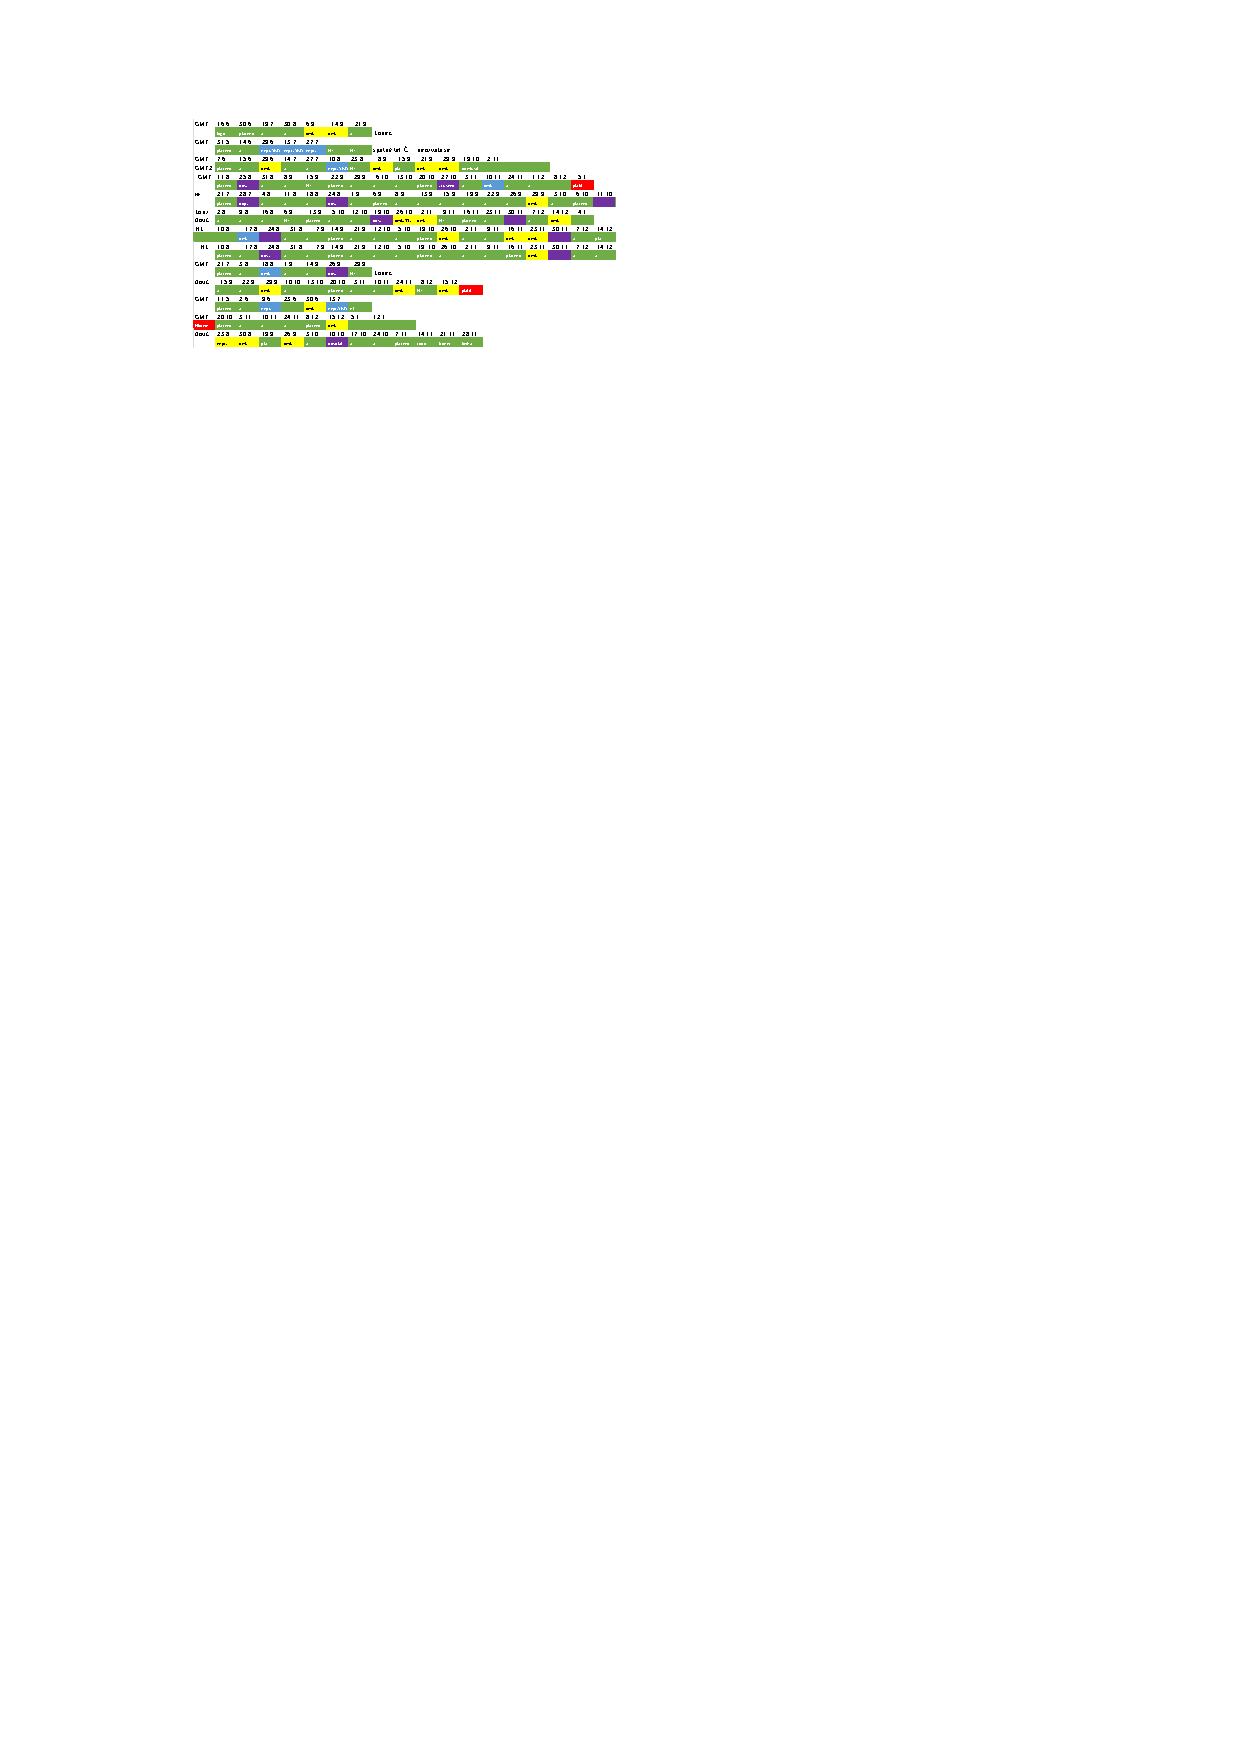
\includegraphics[width=1\textwidth]{img/excel}
    	\caption{Výřez ze stávající tabulky s evidencí klientů}\label{fig:excel}
    \end{figure}
    
    Zpočátku tento způsob evidence samozřejmě fungoval (prakticky okamžitě se mohl bez většího učení a práce začít používat) a dokud nebylo potřeba evidovat historii docházky na jiné kurzy klienta a klientů bylo méně, byl soubor relativně udržitelný. Po několika letech ale situace dospěla do stavu, že je třeba evidovat naráz hodně klientů (běží hodně kurzů, i těch dlouhodobějších) a přidávají se i další informace, které je potřeba evidovat, ale už to není v rámci tabulky možné. Rychlé, ale samozřejmě naprosto neudržitelné řešení, je evidování těchto údajů jinde, byla zvolena papírová forma. Tedy v tabulce jsou vedeny jednotlivé lekce (jen datumy bez času), zda je zaplaceno/předplaceno, zda klient došel, omluvil se, nebo je kurz uzavřený. V papírové formě jsou poté evidovány kontakty na klienta, historie kurzů, konkrétní lekce i s časem.
    
    Pro tuto práci je vhodné si přehledně shrnout nevýhody a výhody tohoto vedení informací a tyto závěry pak zužitkovat při tvorbě webové aplikace, která neduhy vyřeší.
    
        \subsection{Nevýhody řešení}
        \begin{itemize}
            \item \textbf{nepřehlednost:} když klient chodí dlouhodobě, musí se tabulka posouvat vpravo, pak ale nejsou vidět termíny lekcí ostatních klientů, kteří chodí kratší dobu,
            \item \textbf{nekonzistentnost:} nikdo nehlídá, že červená barva nutně znamená zaplatit, v souborech se často objevují chyby, lektorka omylem přepíše data jiného klienta, nemluvě o nekonzistentních textech a barvách (jiný font, velikost, zarovnání, někde napsáno \enquote{placeno} a někde pouze \enquote{pla}) apod.,
            \item \textbf{neefektivní a nekomfortní práce:} pokud má klient více kurzů najednou nebo je potřeba evidovat skupinové lekce, celá evidence je prakticky neudržitelná a je pracné ji udržet v pořádku,
            \item \textbf{chybí historie klienta:} nelze vést přehledně historii kurzů (a příslušných lekcí) klienta, prakticky řešeno tak, že se jednou ročně v září vytvoří nový soubor, kam se překopírují pokračující klienti a připisují se noví klienti, pokud ještě navíc chodí klient na více kurzů v jednom roce, tak se musí složitě rozlišovat jednotlivé lekce,
            \item \textbf{chybí údaje o klientovi:} neevidují se kontaktní a další informace o klientovi, řešeno papírovou evidencí,
            \item \textbf{chybí jiné pohledy:} chybí přehled pro aktuální den a týden a tato informace se nedá ani snadno dohledat, také chybí čas lekce, řeší se papírovým diářem,
            \item \textbf{neresponzivita:} na tabletu se tabulka špatně upravuje, na mobilním zařízení ještě hůře.
        \end{itemize}
        
        \subsection{Výhody řešení}
        \begin{itemize}
            \item \textbf{rychlý rozjezd}: počáteční rozjezd evidence byl rychlý, nebyly potřeba žádné znalosti,
            \item \textbf{žádné poplatky}: lektorka již má Excel nainstalovaný, Dropbox je ve verzi zdarma.
        \end{itemize}
        
        \subsection{Shrnutí}
        Je jasné, že i přes to, že je Excel velmi silný nástroj, tak není vhodný k evidenci tohoto typu. Poskytuje sice další pokročilé funkce, díky kterým by se tato tabulka dala vylepšit, ale stále by nebyla schopna pokrýt veškeré požadavky a potřeby lektorky a také by se rozhodně nejednalo o intuitivní a jednoduchou správu (o těžkopádné editovatelnosti v mobilních zařízeních ani nemluvě).
    
    \section{Podobné aplikace}
    Po pečlivém hledání jsem nenalezl žádnou webovou aplikaci, která by pokrývala alespoň většinu požadavků. Z nalezených aplikací, které se alespoň vzdáleně podobají některým požadavkům lze jmenovat snad jen online nástroj RAYNET.cz, což je cloudový CRM (Customer Relationship Management\footnote{systém pro řízení vztahů se zákazníky pro sledování a vyhodnocování obchodních aktivit v rámci společnosti \cite{crm}}) systém pro řízení vztahů se zákazníky -- poskytuje např. databázi kontaktů, historii vztahu s klientem (schůzky, dokumenty, e-maily, reklamace, poznámky), seznam aktuálních zakázek, obchodní výsledky, kalkulace nabídek, kalendář, spolupráci kolegů, fakturaci \cite{raynet}. Jedná se o moderní, robustní systém, který sice nabízí alespoň nějakou formu evidence klientů s kalendářem a další, ale je nerozšířitelný a nesplňuje z velké části ani funkční požadavky, které jsou specifické a je tedy potřeba vyvinout webovou aplikaci na míru podle potřeb lektorky: jednoduchou, pokrývající všechny požadavky a neobsahující zbytečné funkce navíc.

\chapter{Architektonické vzory ve webových aplikacích}
Než se dostanu k samotnému hledání technologií, je potřeba pochopit, jaké architektonické vzory se ve webových aplikacích používají a proč. V této kapitole nejprve popíši dva vzory, se kterými se u různých webových technologií lze setkat. Díky tomu pak budu moci nalezené technologie v další kapitole rozlišovat i podle vzorů, na kterých jsou postaveny.

Tvorba (nejen) webové aplikace nutně nevyžaduje volbu jakéhokoliv architektonického vzoru, ale je dost pravděpodobné, že bez takovéto berličky bude sice možná aplikace docela fungovat, ale může být hůře rozšířitelná, spravovatelná a pochopitelná. Jakýkoliv zásah pak může vyústit v přepisování kódu celé aplikace (mluvím i ze své zkušenosti).

V poslední části této kapitoly popíši možné přístupy k řešení interakce mezi serverovou a klientskou částí. Díky tomuto rozdělení získám dostatečný přehled k tomu, abych mohl v další kapitole pochopit rozdílné přístupy jednotlivých technologií a rozhodnout se, které možnosti zvolit pro řešení výsledné aplikace.

    \section{MVC a další jeho varianty}\label{mvc}
    MVC (Model-view-controller) vzor dle \cite{mvc-cz1} původně vznikl pro desktopová GUI, ale později se rozšířil zejména mezi vývojáři webových aplikací. Mnoho populárních webových frameworků pro různé jazyky a pro serverovou i klientskou část stojí buď přímo na MVC \cite{mvc-cz1}, nebo využívají jeho odvozeninu: MVP (Model-view-presenter), MVT (Model-view-template) ad. -- souhrnně jsou někdy tyto architektury označovány jako MVW (Model-view-whatever) nebo MV* \cite{mvw}, pro odkazy na tyto technologie v dalším textu budu používat MVW.
    
    \textit{\enquote{MVC vychází z teorie, že části kódu, které vykonávají různé úkoly, by měly být od sebe oddělené.}} \cite{mvc-cz2} Nedodržení tohoto přístupu často pak může i díky absenci disciplíny programátora vést ke špagetovému kódu, vše je smícháno a výsledná aplikace je neudržitelná a těžko rozšířitelná \cite{mvc-cz2,mvc-2}. Díky tomuto rozdělení zodpovědnosti se při vývoji může programátor zaměřit pouze na příslušnou část a kód splňuje principy vysoké soudržnosti a nízké provázanosti \cite{mvc-medium1}. Na druhou stranu je ale třeba říci, že se menší aplikace při použití MVC může stát poměrně robustní, je to ale daň za dekompozici do tří částí a s tím spojené již zmíněné výhody \cite{mvc-medium1}. Další výhodou je možnost mít například více pohledů na stejný model \cite{mvc-1}. Aplikace je, jak je uvedeno v \cite{mvc-cz2}, rozdělena do tří částí:
    \begin{itemize}
        \item modely -- starají se o logiku (výpočty, výsledky, získání a uložení dat, validace), při použití ORM (Object-relational mapping) korespondují modely s tabulkami v databázi,
        \item pohledy -- mají na starost vykreslení stránky v HTML (Hyper Text Markup Language) a JS (Javascriptu), do pohledů jsou nejčastěji pomocí šablonovacího systému dodána všechna potřebná data. Modely se 
        \item kontrolery -- prostředníci mezi modely a pohledy, propojuje je a říká, co vše je potřeba provést pro výsledek.
    \end{itemize}
    
    Jednoduchým příkladem znázorňujícím tento vzor je např. otevření URL \verb|http://domena.cz/uzivatele/15| -- požadavek je zachycen tzv. routerem a na základě parametrů se použije příslušný kontroler, ten zavolá model, který vyhledá daného uživatele v databázi a vrátí jeho údaje kontroleru, který vytvoří pohled a předá mu získaná data \cite{mvc-cz1}.
    
    Jak bylo již naznačeno v úvodu této sekce, existují mírné úpravy MVC vzoru. Tento případ lze ilustrovat na frameworku Django pro Python (podrobněji se tomuto frameworku budu věnovat v podsekci \ref{sec:python}), který využívá MVT. Dle jeho autorů \cite{django-docs-mvp} pohled nepopisuje podobu dat, ale která data (resp. model) na základě URL jsou zobrazena. Jak se zobrazí data je delegováno z pohledu na šablonu, která je tvořena HTML a šablonovacím jazykem. V tomto pojetí nebyl explicitně zmíněn kontroler, ten je tvořen samotným frameworkem, který odešle požadavek na příslušný pohled podle konfigurace. Zkráceně lze tedy říci, že programátor poskytne model, pohled a šablonu, které poté sváže s příslušnou URL a o zbytek se postará Django \cite{django-mvp2}.
    
    \section{CBA}\label{cba}
    V posledních letech nastal poměrně velký zlom v oblasti frameworků pro klientskou část aplikací. Vznikají nové a nové javascriptové frameworky a ty již zaběhlé se přizpůsobují poptávce a často radikálně mění své přístupy k architektuře (např. Angular, viz. podsekce \ref{sec:angular}). Více a více se na straně klienta upouští od architektur MVW mj. z důvodu velmi úzké svázanosti kontroleru a pohledu a také porušování principu jedné odpovědnosti\footnote{jedno z pravidel objektově orientovaného programování -- každý objekt by měl mít jen jednu odpovědnost (tedy jediný důvod ke změně) \cite{single-responsibility}} (protože se kontroler stará jak o logiku, tak o zpracování událostí) \cite{mvc-frontend}.
    
    Vývoj vyústil ve využití v tomto odvětví doposud nepoužívané architektury CBA (Component-Based Architecture) a s tím spojených  \enquote{unidirectional} architektur (tedy architektur pro jednostrannou komunikaci ke spravování stavu aplikace). Tyto architektury dokáží nejen pokrýt klasický MVW přístup, ale poskytují i mnohem lepší oddělení odpovědnosti \cite{mvc-frontend}.
    
    CBA je podle \cite{cba3} založeno na rozdělení částí kódu na jednotlivé nezávislé, snadno testovatelné, rozšiřitelné a znovupoužitelné komponenty (v tomto případě tvořící UI), které obsahují všechny potřebné závislosti. Komponenta zapouzdřuje svou funkcionalitu a chování a zároveň navenek poskytuje jednotné rozhraní pro přístup. Díky komponentám tak může být tvorba nebo úprava UI rychleji hotová (lze používat např. i komponenty od jiných autorů) a je zajištěna konzistence napříč celou aplikací. Dalším uplatněním komponent je například jejich souvislost s procesy analýzy požadavků a návrhu během tvorby aplikace, kdy se při přidávání funkcí nemusí zdlouhavě popisovat samotná komponenta a pak teprve její rozšíření, ale stačí definovat pouze rozšiřující funkce \cite{cba1}. Použití komponent také pomáhá dodržet princip DRY (\enquote{Don't repeat yourself}) \cite{cba2}.
    
    \section{Interakce mezi serverovou a klientskou částí}\label{interakce}
    Cílem této sekce je ukázat aktuální možnosti řešení interakce mezi serverovou a klientskou částí. Díky tomu, že jsou weby mnohem interaktivnější než dříve, nebylo už často možné úzce svazovat klientskou a serverovou část a bylo potřeba je oddělit prostřednictvím API. To vše v této sekci představím.
    
        \subsection{Skriptování na straně serveru}
        Webové aplikace byly typické využíváním skriptování na straně serveru \cite{moderni-webapps}, tedy na základě požadavku byl na webovém serveru připraven HTML soubor, který byl poté odeslán do klientova prohlížeče \cite{scripting-sqa} (viz. příklad Djanga na konci sekce \ref{mvc}). Používání tohoto způsobu samostatně se hodilo a hodí zejména pro stránky, které například přímo spolupracují s databází, vrací texty a obrázky, ale nevyžadují příliš interaktivity \cite{scripting-freecodecamp}.
        
        \subsection{Skriptování na straně klienta}\label{client-side-scripting}
        S trochou nadsázky by se, jak říká autor v \cite{scripting-freecodecamp}, dalo říci, že dnes jsou webové stránky spíše aplikace předstírající, že jsou stránky -- web je mnohem pokročilejší než dříve, umožňuje chatování, nakupování, prohlížení aktuálního proudu novinek atd. To znamená mnohem větší zátěž na server, který vše musí obstarat. Pro pokročilejší interaktivní aplikace bylo tedy potřeba začít ve větší míře začít používat Javascript, který umožní určitou část zátěže přenést na klientskou část \cite{scripting-upwork} a skriptování na serveru doplnit o skriptování na straně klienta, tedy v prohlížeči. Je ale potřeba říci, že robustní aplikace využívající skriptování na straně klienta může být složitější implementovat, oproti těm využívající především skriptování na straně serveru \cite{scripting-fasthosts}.
        
        Vývoj dnes pokročil až do situace, že pro pokročilé možnosti interaktivity byly připraveny přímo JS frameworky \cite{scripting-upwork}, server tedy prakticky jen odešle jednoduchý HTML soubor s odkazy na Javascriptové knihovny, které obstarají zbytek práce u klienta a obsah stránky dynamicky generují a komunikují se serverem, od kterého obdrží pouze potřebné informace bez zbytečné režie navíc ve formě HTML tagů a struktury celé stránky \cite{scripting-fasthosts}. Tyto frameworky obvykle pracují s API (Application Programming Interface, blíže popíši v podsekci \ref{api}) a AJAX (Asynchronous JavaScript and XML)\footnote{technologie pro asynchronní přenos dat na pozadí bez potřeby načíst celou stránku \cite{scripting-fasthosts}} dotazy \cite{scripting-fasthosts} a představují tak jednoduchou možnost okamžité a efektivní asynchronní komunikace se serverovou částí \cite{scripting-upwork}. Podobných výsledků lze dosáhnout i bez JS frameworků a explicitně vytvořeného API, jak uvádí např. autor v \cite{scripting-simpleis} -- jednotlivé pohledy s pomocí šablon na serverové straně vrací buď klasicky celou stránku a nebo pouze JSON, tyto jsou pak využity pro AJAX volání v JS na straně klienta, tento přístup se ovšem hodí pro méně interaktivní aplikace. AJAX a další operace v JS také zaznamenaly zvýšení popularity i díky knihovně \href{http://jquery.com/}{jQuery}, která přinesla značné zjednodušení práce s JS \cite{scripting-upwork}.
        
        Nevýhodou skriptování na straně klienta je samozřejmě nutnost mít povolený příslušný skriptovací jazyk (tedy většinou Javascript) \cite{scripting-sqa}. Dalším potenciálním problémem může být prvotní čas načtení stránky, především JS souborů, a s tím spojený problém se SEO (Search Engine Optimization)\footnote{optimalizace nalezitelnosti na internetu \cite{seo}}, pokud není aplikace implementována korektně nebo její načtení trvá déle (roboti obdrží prázdnou stránku s načítací animací a nemusí vědět, že mají čekat na její načtení) \cite{scripting-freecodecamp,scripting-hackernoon}. Tento klasický přístup bývá obvykle nazýván jako CSR (Client-Side Rendering) a je obvykle frameworky v základu používán. Na přelomu roku 2016 a 2017 se tak začaly objevovat řešení umožňující SSR (Server-Side Rendering), např. balíček \href{https://github.com/angular/universal}{Angular Universal}, mini-framework \href{https://github.com/zeit/next.js/}{next.js} pro React \cite{scripting-hackernoon}. Díky těmto dodatečným úpravám je, jak je ukázáno v \cite{scripting-ytb}, aplikace vykreslena na serveru a ve formě stringu je do výchozí kostry HTML vložen předvykreslený kód komponenty a takovýto HTML soubor je zaslán klientovi, který tak vidí bez prodlení stránku a její obsah a pouze čeká na načtení JS, aby byla stránka interaktivní, další interakce v aplikaci pak už probíhají klasicky ve stylu CSR prohlížečem. Tento přístup ale nutně nemusí znamenat zrychlení výkonu a načítání, pokud je například string, který se vygeneruje na serveru velmi dlouhý, dojde naopak ke zvýšení velikosti přenášeného HTML souboru ke klientovi a zvýšení zátěže serveru (kvůli které se na CSR přechází) a tím v důsledku použití SSR naopak ke zpomalení načítání \cite{scripting-hackernoon}. Při využití SSR je tedy potřeba brát v úvahu mnoho faktorů, mimo již zmíněných také finance a s tím související výkon serveru (server bude více zatížený a nemusí být tolik výkonný), v úvahu také připadá kromě řešení teoretických věcí i praktické testování obou přístupů, tento přístup například zvolili vývojáři v \cite{scripting-benchmark} a po vyhodnocení výsledků pro většinu stránek zvolili SSR.
        
        Na závěr si ještě dovolím menší vsuvku k terminologii, skriptování na straně klienta a serveru je často zaměňováno za renderování a naopak (dokonce je i občas špatně interpretován smysl renderování JS na serveru \cite{scripting-chyby}), někteří autoři tyto termíny považují za stejné \cite{scripting-freecodecamp}, ale pro tuto práci je vzhledem k tomu, že se častěji opravdu používají v odlišných souvislostech, považuji za odlišné. Renderování (tedy CSR a SSR) je obvykle spojováno pouze s JS frameworky a předvykreslením stránky díky skriptování na straně serveru, kdežto skriptování na straně klienta a serveru je obecně spojováno se všemi možnými jazyky.
    
        \subsection{API}\label{api}
        Obecně uznávanou praxi při vytváření moderní webové aplikace (zejména s JS frameworkem a SPA, viz. další podsekce \ref{spampa}) je zaslání úvodní stránky od serveru ke klientovi a poté načítání a ukládání dat prostřednictvím jednoduchých zpráv z klienta, neboli prostřednictvím definovaného rozhraní API \cite{api1}. 
        Takové rozhraní poskytuje konzistentní, univerzální a flexibilní možnost sdílení dat a funkcionality napříč různými technologiemi a systémy \cite{api2}. Klientská a serverová část jsou od sebe odděleny a jsou na sobě prakticky nezávislé, změna na jedné straně (např. v databázi) by neměla vyvolat nutnost změny na straně druhé \cite{api3} -- například lze snadno vyměnit GUI (JS framework) a použít jiné prakticky bez nutnosti zasáhnout do logiky a funkcionality na serveru.
        
        Ve webových aplikacích se velmi často používá REST (Representational State Transfer) API \cite{api1}. Tato architektura podle \cite{api4} umožňuje přistupovat k datům na určitém místě (každý zdroj má jeden koncový bod, na který přistoupíme) pomocí metod HTTP (Hypertext Transfer Protocol): GET (získání dat), POST (vytvoření), PUT (úpravy celého zdroje), DELETE (smazání), PATCH (částečné úpravy) a provádět nad nimi CRUD (create-read-update-delete) operace. Součástí HTTP jsou i stavové kódy, na základě požadavku tak součástí odpovědi jsou dle \cite{api4} stavové kódy, například:
            \begin{itemize}
                \item \textbf{200 OK}: požadavek byl úspěšně proveden,
                \item \textbf{201 Created}: nový obsah byl vytvořen (pro POST),
                \item \textbf{400 Bad Request}: požadavek je nečitelný (např. špatný formát zaslaných dat),
                \item \textbf{401 Unauthorized}: požadavek není autorizován,
                \item \textbf{404 Not Found}: zdroj nenalezen,
                \item \textbf{405 Method Not Allowed}: zdroj není dostupný pro tuto metodu.
            \end{itemize}
        Podle \cite{api5} se REST spolu s JSON (JavaScript Object Notation) stává defacto standardem pro API webových služeb a spolu s frameworky pro vývoj aplikací na straně serveru poskytuje snadnou možnost jak si vytvořit vlastní REST rozhraní. JSON je formát pro výměnu dat, který se zařadil mezi nejdůležitější formáty na webu. Jeho úspěch tkví v tom, že se s ním díky zápisu dat v souladu s JS pracuje v oblasti zápisu krátkých strukturovaných dat mnohem lépe než s konkurenčním XML (eXtensible Markup Language) \cite{api6}.
        
        \subsection{SPA a MPA}\label{spampa}
        V současné době existují dvě možnosti, jak implementovat procházení jednotlivých stránek webovou aplikací: SPA (Single-Page Application) a MPA (Multi-Page Application). Obě tato řešení krátce představím a uvedu jejich výhody, nevýhody a použití.
        
        MPA je podle \cite{spa1} označení pro tradiční způsob známý již od prvních webových stránek, tedy každá změna vyvolá vykreslení nové stránky v prohlížeči (tedy v panelu prohlížeče se zobrazí např. načítací kolečko, dokud není přenos nové stránky ze serveru dokončen). Využívá se především pro stránky, které mají mnoho úrovní v menu, tedy jsou co se týče struktury velmi rozmanité a bohaté, dále velmi dobře fungují co se týče SEO. Nevýhodou může být úzké propojení mezi klientskou a serverovou částí. MPA nevyžaduje z podstaty věci žádné dodatečné technologie a je velmi jednoduché takovouto aplikaci vytvořit (oproti SPA).
        
        SPA je podle \cite{spa1} aplikace, která běží přímo u klienta v prohlížeči a nevyžaduje při procházení jakékoliv znovunačítání (indikované samotným prohlížečem), tento způsob používá např. \href{https://www.facebook.com/}{Facebook}, \href{https://mail.google.com/}{Gmail}, \href{https://www.google.com/maps}{Google Mapy}, \href{https://www.stream.cz/}{Stream}, \href{https://jizdenky.arriva.cz/}{e-shop Arriva} ad. Díky této vlastnosti lze poskytnout uživateli vynikající UX (User Experience\footnote{celkový prožitek z používání např. webové aplikace \cite{ux}}), protože se najednou aplikace chová přirozeně, neproblikává při přechodu mezi stránkami, prohlížeč neukazuje v panelu načítání -- uživatel je stále v jednom prostoru a cítí se tak pohodlně. Aplikace vlastně napodobuje desktopové programy, kde také nedochází k načítání při přechodech \cite{spa2}. Autorka v \cite{spa2} dokonce přímo píše: \enquote{\textit{Nothing beats user experience offered by SPA.}} Mezi další výhody SPA dle \cite{spa1} a \cite{spa2} patří:
        
        \begin{itemize}
            \item rychlé přecházení mezi stránkami -- většina zdrojových souborů (HTML, CSS, skripty) je načtena pouze na začátku a během přechodů tak dochází pouze k posílání a přijímání dat jako takových (informace z databáze apod.),
            \item jednoduchá výměna klientské části (která se v praxi mění častěji) při zachování stejné serverové části,
            \item možnost znovupoužití kódu serverové části pro nativní mobilní aplikaci, protože veškeré přechody mezi stránkami (kromě zaslání úvodní stránky ze serveru) jsou spravovány na straně klienta a ne serveru, jako v případě MPA -- server poskytuje pouze API, které se právě se SPA používá,
            \item snadnější tvorba offline aplikací.
        \end{itemize}
        
        Pro jednoduchou implementaci SPA se používají JS frameworky, z čehož plyne samozřejmě požadavek na zapnutý JS u uživatele. Také je potřeba počítat s delším prvotním načtením (kód aplikace je delší), už jsem ale zmínil řešení pomocí SSR (viz. sekce \ref{interakce}). Dalším potenciálním problémem ve SPA aplikaci je nekorektní odchycení problému, kvůli kterému může dojít ke znemožnění ovládání celé aplikace a minimálně je ji potřeba znovu načíst.

\chapter{Volba technologií}\label{technologie}
Důležitou volbou při tvorbě aplikace jsou technologie. Odvětví webových aplikací je oproti jiným specifické především svou rychlostí rozvoje. Díky tomu, že jsou webové technologie stále populárnější (například pro svou nezávislost na platformě), rostou i další požadavky programátorů a s tím ruku v ruce vzniká nepřeberné množství dalších technologií, frameworků a knihoven \cite{moderni-webapps,moderni-webapps2}. Cílem této kapitoly je poskytnout ucelený základní přehled technologií používaných v současné době pro tvorbu webových aplikací a jejich provozování. Nejprve představím možnosti řešení na straně klienta a serveru, poté zmapuji oblast databází a srovnám hostingy pro provozování výsledné aplikace a v závěrečné části zvolím řešení pro připravovanou aplikaci ÚP.

Ještě před začátkem si dovolím jednu poznámku. Jak uvádí autoři v \cite{technologie1}, výběr technologií pouze na základě procházení článků a srovnání je velmi ošemetný a často bude programátor stát na rozcestí, kde budou proti sobě stát dva autoři se svými tvrzeními, která se budou navzájem vylučovat a občas nemusí být snadné najít bez hlubších znalostí a zkušeností to pravdivé. Při popisu technologií (a zároveň pak i výběru) tedy budu klást důraz, jak je řečeno v \cite{technologie1} a \cite{technologie2}, na účel a požadavky na aplikaci, snadnost a jednoduchost řešení (např. existenci nástrojů umožňujících rychlý start, tzv. \enquote{starter boilerplates}), ekosystém a komunitu kolem dané technologie (čím více lidí, tím je pružnější vývoj, vzniká více knihoven a objeví se více otázek a odpovědí), kvalitní dokumentaci, dospělost (začínající technologie může změnit svůj směr) a také na to, kdo za technologií stojí.

Občas budu uvádět také data z některých průzkumů, aby bylo jasné, nakolik jsou vypovídající, uvádím zde, na jakém vzorku byly prováděny:
\begin{itemize}
    \item průzkum Stack Overflow \cite{stack-stats17} na přelomu ledna a února 2017 absolvovalo přes 64~227~vývojářů z 213~zemí, z toho 70~\%~zaměstnaných na plný úvazek,
    \item průzkum Stack Overflow \cite{stack-stats18} v lednu 2018 absolvovalo přes 101~592~vývojářů ze 183~zemí, z toho 74~\%~zaměstnaných na plný úvazek,
    \item průzkum Jetbrains \cite{jetbrains-stats} na přelomu roku 2016 a 2017 absolvovalo přes 9~000 vývojářů z 20~zemí, z toho 67~\%~zaměstnaných ve firmě či organizaci.
\end{itemize}

    \section{Klientská část}
    V této části popíši základní technologie, které se používají při tvorbě webových aplikací: HTML, CSS a JS. Jak už jsem zmínil v podsekci \ref{spampa}, pro pokročilejší interakci a SPA se volí JS frameworky a knihovny, nejprve uvedu dříve velmi často používanou knihovnu jQuery, poté se zaměřím přímo na aktuální frameworky a knihovny. Pochopit rozdíly v tak rychle měnícím se prostředí je náročné (frameworky mění během svých verzí i celou architekturu), informace tak snadno zastarají, stejně jako samotné aplikace. Jedním z aktuálních a velmi dobře hodnocených článků je \cite{js-fw2}, kde autor velmi rozsáhle shrnuje výhody a nevýhody jednotlivých frameworků. Cílem této práce není ale hloubková analýza všech frameworků, proto se zaměřím na jejich základní popis a výtah z některých článků, aby bylo jasné, čím se frameworky odlišují.
    
    Pro úplnost dodávám, že výčet frameworků zdaleka není úplný, z důvodů uvedených před touto částí v kapitole \ref{technologie} jsou zvoleny tři v současné době nejpopulárnější podle \cite{hot-frameworks} (seřazeno podle průměru z počtu hvězdiček na GitHub a počtu otázek na Stack Overflow). Pro představu o jejich popularitě ve vyhledávání Google přikládám obrázek \ref{fig:js-frameworks} aktuálního grafu s trendy (je na místě poznamenat, že terminologie kolem verzování Angularu je mírně krkolomná, což je vidět zejména před rokem 2016, kdy existoval jen AngularJS a přesto byl Angular vyhledáván, dále \enquote{vue} je obecné slovo široce užívané i mimo JS frameworky, z toho důvodu je zvolen jako vyhledávací dotaz \enquote{vuejs}, což mohlo mírně tomuto frameworku uškodit).
    
    \begin{figure}[!hb]\centering
    	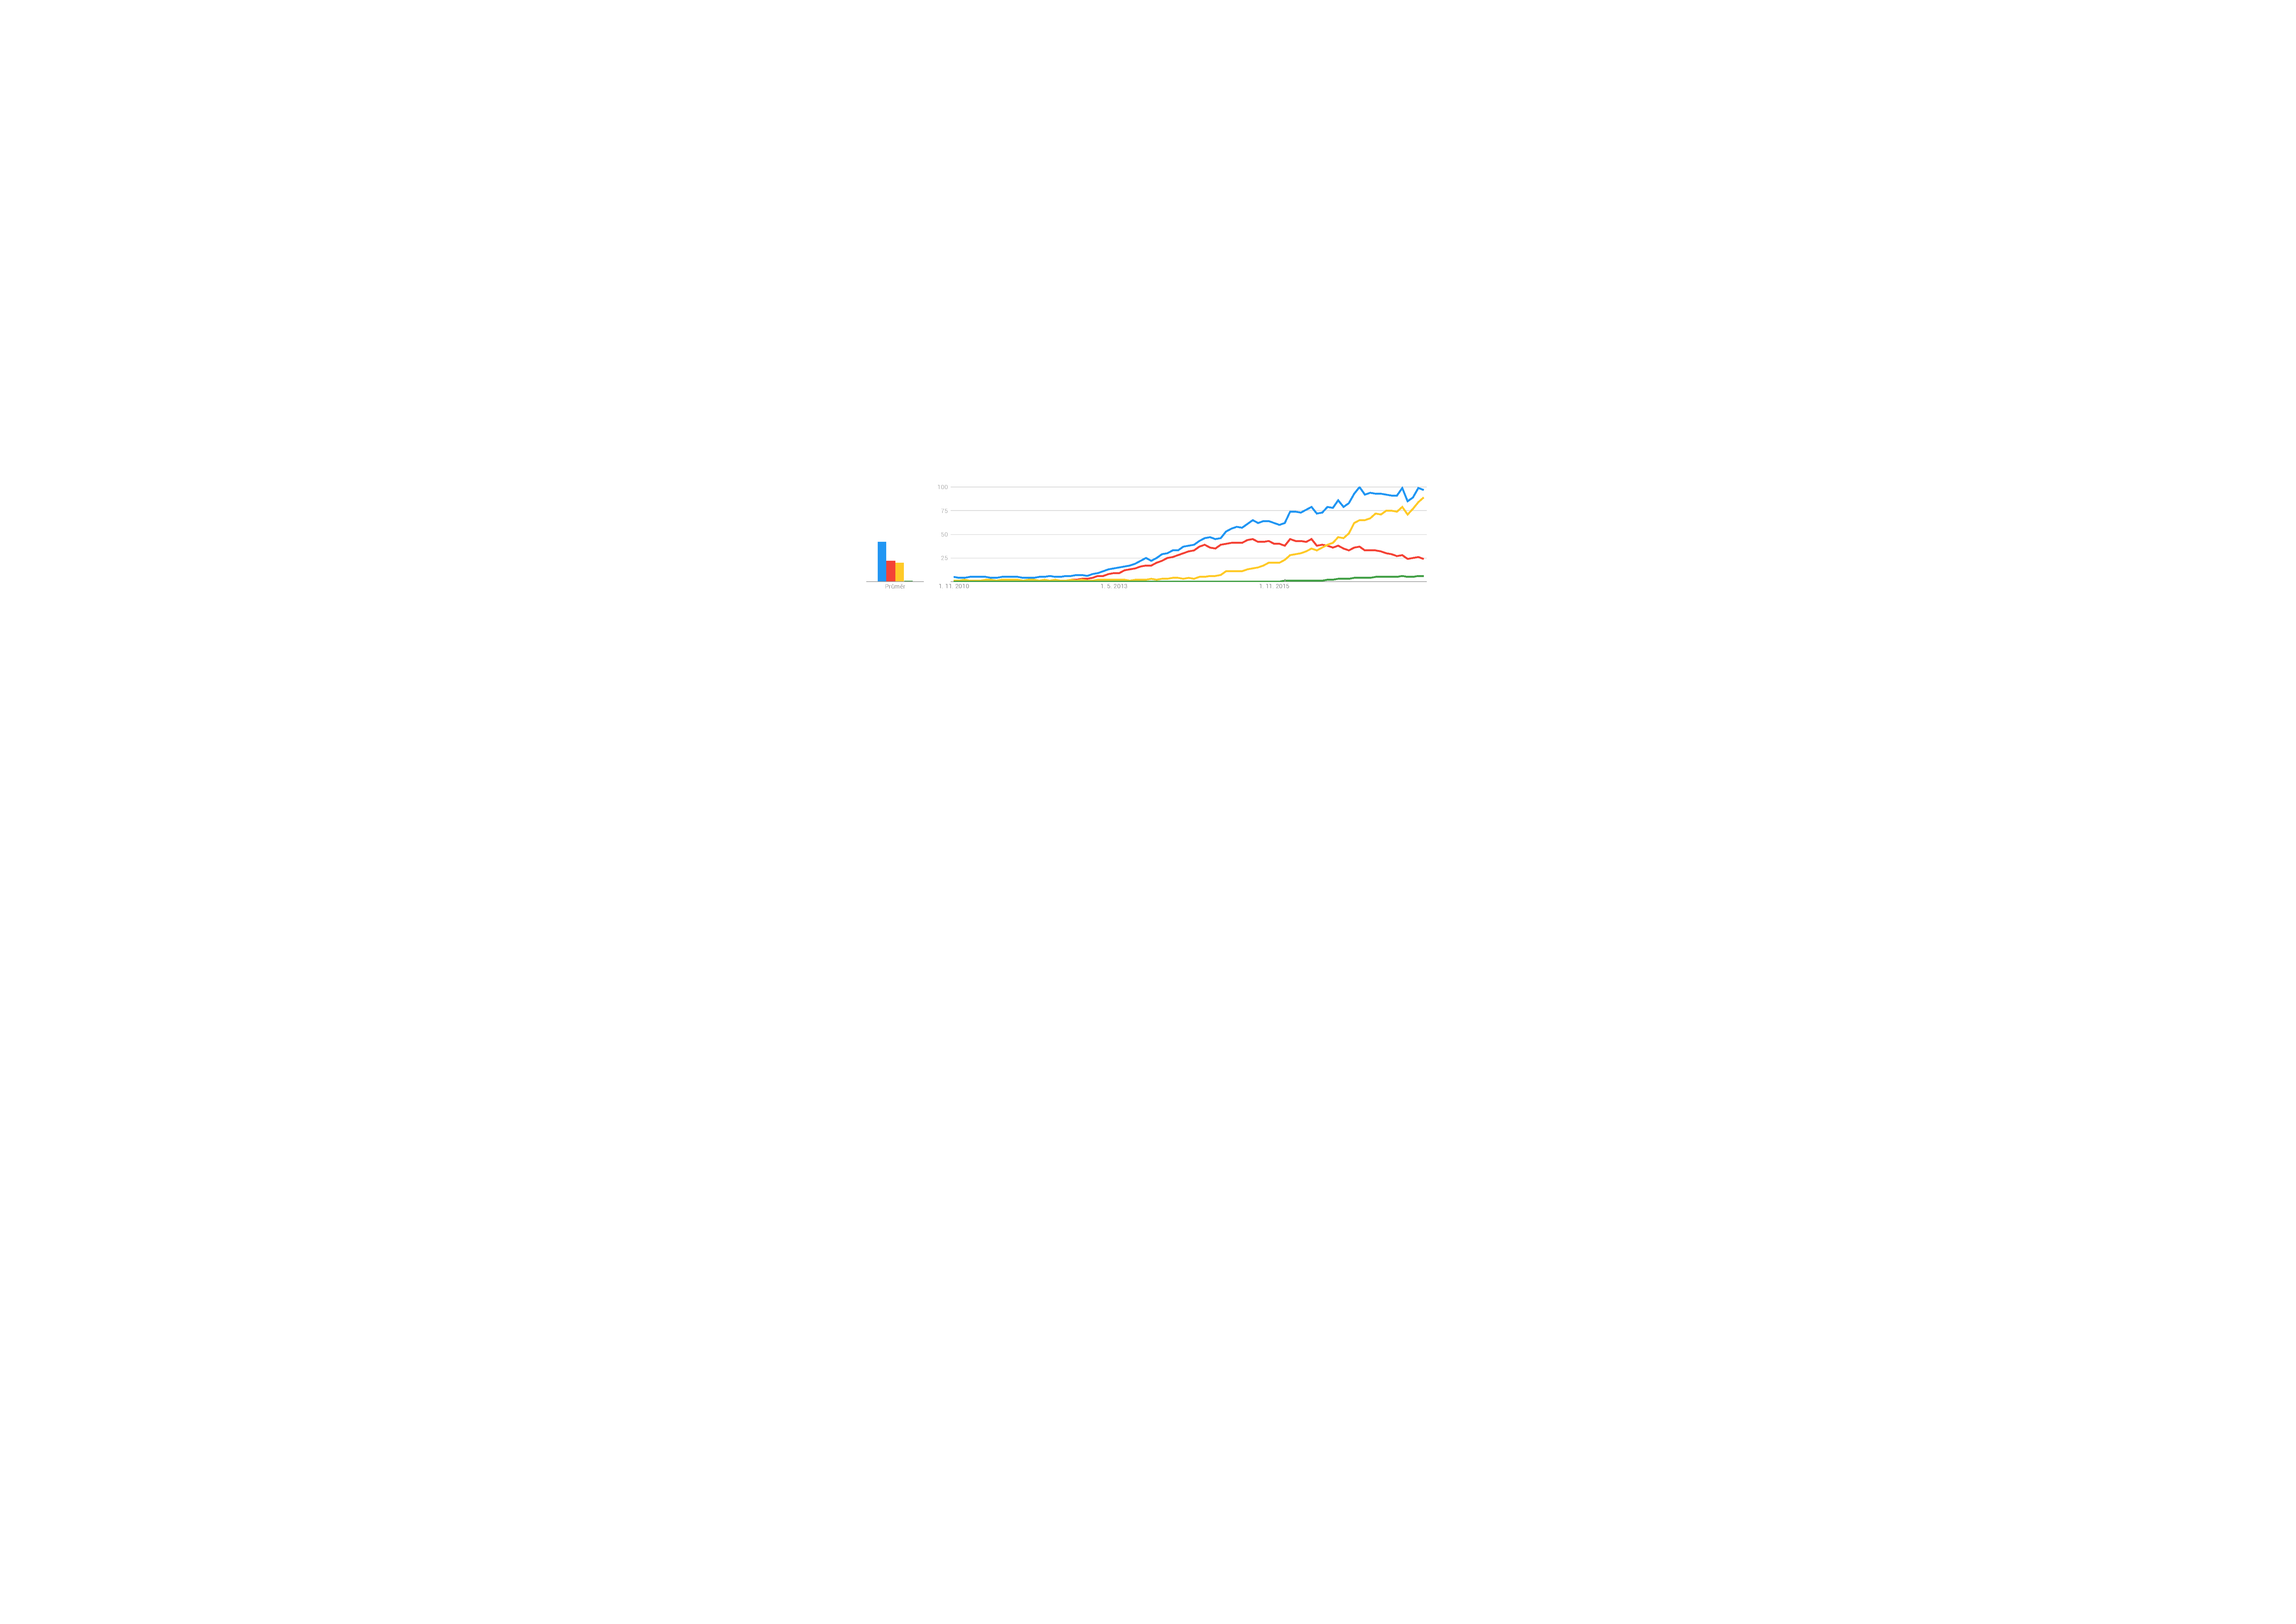
\includegraphics[width=1\textwidth]{img/js-frameworks}
    	\caption[Popularita JS frameworků ve vyhledávači Google]{Celosvětová popularita JS frameworků ve vyhledávači Google od 20.~10.~2010 do 31.~3.~2018 v kategorii Počítače a Elektronika -- modře \textit{angular}, červeně \textit{angularjs}, oranžově \textit{react}, zeleně \textit{vuejs} \cite{trends-google}}\label{fig:js-frameworks}
    \end{figure}
    
        \subsection{HTML a CSS}
        HTML (Hyper Text Markup Language) je značkovací jazyk, bez kterého se dnes při tvorbě webové aplikace nedá obejít, popisuje strukturu webové stránky pomocí HTML značek \cite{html1}. V současné době je aktuální používání HTML5, které přináší spoustu dlouho očekávaných funkcí pro moderní web \cite{html2}, je třeba ale brát na vědomí stále ještě neúplnou podporu všech novinek ze strany všech prohlížečů \cite{html3}.
        
        CSS (Cascading Style Sheets) je jazyk pro zápis způsobu zobrazení elementů HTML stránky \cite{css2}. V současné době se používá CSS3, které přineslo mj. možnost jednoduše vytvářet responzivní stránky, animace a přechody \cite{css3}. Stejně jako u HTML5 je třeba brát v úvahu neúplnou podporu všech novinek ze strany všech prohlížečů \cite{css1}.
        
        \subsection{Javascript, jQuery}\label{js}
        Javascript je skriptovací interpretovaný jazyk, který se obvykle používá pro skriptování na straně klienta (na straně serveru viz. podsekce \ref{nodejs}) -- pro jakoukoliv interakci a animace na stránce \cite{js2}. Během let se stala mezi programátory velmi populární knihovna jQuery (padla o ní řeč už v podsekci \ref{client-side-scripting}), která výrazně zjednodušuje a zaobaluje syntaxi JS \cite{scripting-upwork}. JS je nejpoužívanější jazyk vycházející ze specifikací ECMAScript, v posledních letech díky implementaci specifikací ECMAScript 5, 5.1, 6, 7 a 8 obdržel spoustu důležitých funkcionalit a syntaktické nadstavby včetně tříd \cite{js3}.
        
        Opět je zde samozřejmě problém s kompatibilitou v prohlížečích, to se ale obvykle řeší použitím transpileru (překladač mezi dvěma jazyky na stejné úrovni abstrakce) Babel, který může kromě transpilace poskytnout i polyfilly (nahrazují nativní API prohlížeče) \cite{js4,js1}. Další často používanou nadstavbou pro větší JS aplikace jsou jazyky jako TypeScript, CoffeeScript \cite{js5} nebo rozšíření JSX (aby HTML v JS vypadalo jako HTML, ačkoliv se jedná o prosté JS funkce \cite{js-fw3}) \cite{js6}.
        
        \subsection{Angular, AngularJS}\label{sec:angular}
        Angular a AngularJS jsou JS frameworky od Google. AngularJS byl, jak je uvedeno v \cite{angular1}, vytvořen v roce 2009 a stavěl na technologii MVC, postupem času se ale začalo ukazovat, že je potřeba použít spíše CBA (viz. sekce \ref{cba}) a změnit přístup i v jiných oblastech. 
        
        V roce 2016 byl tak vydán Angular, později nazývaný Angular 2, vzhledem ke zpětné nekompatibilitě a mnoha změnám i v dalších verzích \cite{js-fw2} se to z některých stran nesetkalo s kladným přijetím \cite{angular2,js-fw1}. Nabízí bohatou knihovnu včetně API pro HTTP požadavky ad., používá Typescript (popsaný v předchozí podsekci \ref{js}).
        
        \subsection{React}\label{react}
        React je podle \cite{react} knihovna (ne framework, viz. další rozebrání v \cite{js-fw1}) od Facebooku, která umožňuje budovat interaktivní uživatelská prostředí. Oproti Angularu je React velmi jednoduchý a malý, protože neobsahuje prakticky žádné dodatečné funkce, v tom spoléhá na komunitu \cite{js-fw1}, tedy například i pro HTTP požadavky je zde potřeba najít a zvolit vhodnou knihovnu, jinak lze použít pouze běžnou JS syntaxi. Pro tvorbu HTML lze volitelně použít JSX (popis viz. podsekce \ref{js}), je to výhodné zejména z důvodu jednoduššího a přehlednějšího zápisu.
        
        \subsection{VueJS}
        VueJS by se s trochou nadsázky dal označit za kombinaci Angularu a Reactu \cite{js-fw5}, z obou přináší skvělé věci a je velmi kladně hodnocen lidmi, kteří před ním pracovali s Angularem nebo Reactem \cite{js-fw1}. Nevýhodou je zatím jeho menší rozšířenost a používanost \cite{js-fw1} a také fakt, že za ním nestojí firma, ale jednotlivec, i z toho důvodu jsou zatím ze strany firem zatím upřednostňovány React a Angular \cite{js-fw4}, jeho popularita se ale pomalu zvyšuje a objevují se týmy, které ho na své větší projekty reálně používají \cite{js-fw1}.
    
    
    \section{Serverová část}
    Volba programovacího jazyka pro serverovou část jde často ruku v ruce s volbou frameworku pro příslušný jazyk. Cílem této části je uvést nejpoužívanější řešení pro webové aplikace včetně možností frameworků. Pro úplnost opět dodávám, že výčet technologií není úplný, podrobněji se nezaobírám např. jazyky C++, Go, Perl a příslušnými frameworky, a to především buď z důvodu velmi specifických možností využití \cite{technologie-c++} nebo menší rozšířenosti \cite{stack-stats18,jetbrains-stats}. Ze stejných důvodů také volím pouze nejpopulárnější frameworky podle \cite{hot-frameworks}.
    
    \begin{figure}\centering
    	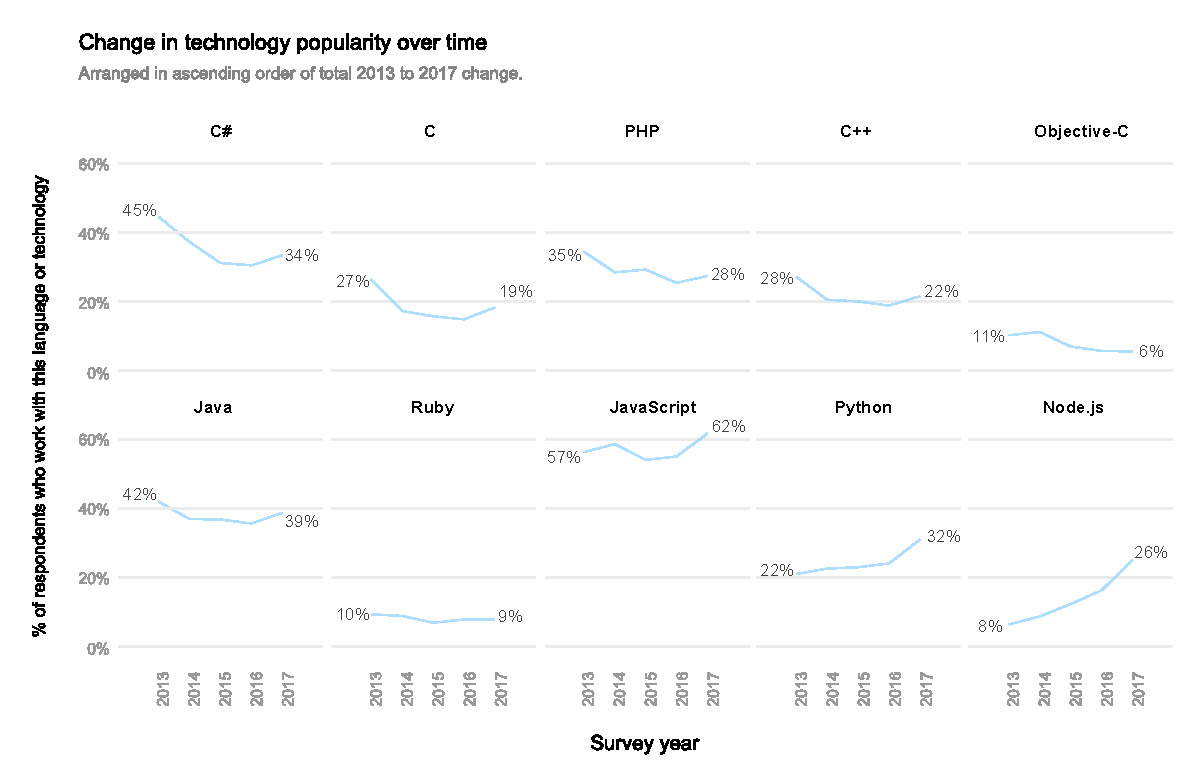
\includegraphics[width=1\textwidth]{img/stack-stats}
    	\caption[Popularita technologií mezi lety 2013 a 2017 dle průzkumu Stack Overflow]{Popularita technologií mezi lety 2013 a 2017 dle průzkumu Stack Overflow, procenta uvádí počet respondentů pracujících s daným jazykem či technologií \cite{stack-stats17}}\label{fig:stack-stats17}
    \end{figure}
    
        \subsection{PHP}
        PHP je slabě typovaný jazyk, který se obvykle používá pouze ve světě webu \cite{tech-python1}. Podle \cite{tech-php1} jej využívá přes 80~\%~webů. Výhodou PHP oproti všem ostatním jazykům je nepřeberné množství levných či bezplatných hostingů s PHP \cite{tech-python4} (například velmi populární tuzemský hosting \href{https://www.endora.cz/}{Endora}) a také dostupnost nejpopulárnějšího CMS (Content Management System) Wordpress (taktéž napsaného v PHP) \cite{tech-python2}.
        
        Hlavní výhodou PHP je možnost snadno a jednoduše začít tvořit webovou aplikaci i bez frameworku, to je ale i hlavní nevýhoda, protože mnoho programátorů pak píše špagetový kód a takové aplikace jsou téměř neudržovatelné \cite{tech-php2}. I z těchto důvodů se často dle \cite{tech1} používají frameworky, kterých je oproti jiným jazykům pro PHP mnohem více, např. Laravel, Zend, Symfony a také tuzemský Nette. Často zmiňovanými nevýhodami jsou např. poměrně nezorganizovaná standardní knihovna \cite{tech-python1}, názvosloví funkcí a nepohodlná práce při použití UTF-8 \cite{tech-php3}.
        
        \subsection{Java}
        Java je jazyk obecně používaný jak pro webové, mobilní, tak desktopové aplikace, často se používá pro rozsáhlé podnikové systémy díky bezpečnosti a výkonu \cite{tech2}. Dle \cite{tech-php1} je Java třetí nejpoužívanější technologie na straně serveru. Pro webové aplikace nabízí mnoho nástrojů a frameworků, např. Spring MVC, Play, JSF, Google Web Toolkit ad. Zde vyzdvihnu framework Play, který umožňuje stavět jednoduché aplikace v jazycích Java nebo Scala a je vhodný i menší projekty (oproti některým jiným frameworkům \cite{tech-java1}) \cite{tech-java2}.
        
        \subsection{C\#}
        C\# je jazyk s širokým použitím pro vytváření bezpečných a robustních aplikací, aplikace (a dále zmiňované frameworky) pak běží na platformě .NET Framework na Windows nebo na multiplatformním .NET Core \cite{tech-csharp1}. Dle \cite{tech-php1} je ASP.NET druhá nejpoužívanější technologie na straně serveru. V roce 2016 Microsoft vydal nový moderní framework ASP.NET Core, který spojuje starší frameworky ASP.NET MVC a ASP.NET Web API \cite{tech-csharp1}. I díky robustnosti celého prostředí se často používá v korporátním prostředí \cite{tech-csharp3}. 
        
        \subsection{Ruby}
        Ruby je jazyk se zajímavou a jednoduchou syntaxí a silným objektovým založením \cite{tech-ruby1}.
        Používá se ve spojení s frameworkem Ruby on Rails, díky kterému je velmi jednoduché začít a po chvíli programování vidět výsledky \cite{tech1}. Práce s frameworkem je postavena na mnoha návrhových vzorech a konvencích, což někteří považují za výhodu \cite{tech1} a jiní za nevýhodu \cite{tech-ruby2}.
        
        \subsection{Python}\label{sec:python}
        Python je silně typovaný jazyk, vyniká především svou jednoduchou syntaxí a srozumitelnou standardní knihovnou s dobrou organizací \cite{tech-python1}, jedná se o obecný jazyk a i díky dostupnosti velkého množství knihoven (např. pro strojové učení a umělou inteligenci) je velmi populární \cite{tech-python3}. Aktuálně je ve verzi 3, která je záměrně zpětně nekompatibilní s verzí 2 -- dle autora jazyka je cílem napravit hříchy jazyka z minulosti \cite{tech-python6}. Jak je vidět na obrázku \ref{fig:stack-stats17}, jeho popularita se stále zvyšuje.
        
        Python se původně se pro webové aplikace vůbec nepoužíval, pro jednoduché vytvoření webové aplikace je potřeba použít některý z webových frameworků, nejpopulárnější je Django a Flask \cite{tech-python4}. Tyto frameworky lze od sebe snadno rozlišit, jak uvádí \cite{tech-python5}: Flask je jednoduchý modulární framework a je na uživateli, jaké součástí si do něj přidá, naproti tomu Django je tzv. \enquote{batteries included} framework, tedy má v sobě spoustu nástrojů, díky kterým může uživatel rychle vyvíjet webovou aplikaci bez nutnosti zabývat se volbou a hledáním konkrétních modulů.
        
        \subsection{Node.js}\label{nodejs}
        Node.js je podle \cite{tech1} prostředí pro efektivní běh JS na straně serveru, díky JS hojně využívá model událostí a asynchronních operací pro maximalizaci výkonu a minimalizaci režie procesoru. Ideou autorů bylo sjednocení jazyka serverové a klientské části, protože moderní aplikace obvykle stály na použití JS na klientovi, ale ne na serveru. 
        
        Popularita Node.js, jak je vidět na obrázku \ref{fig:stack-stats17}, strmě roste, na druhou stranu se ale objevují názory \cite{tech-node1}, že JS patří pouze na stranu klienta. Pro jednodušší vývoj webových aplikací se často používá framework Express \cite{tech-node2}. I když programátor zvolí na server jinou technologii, často se i tak s Node.js setká např. ve formě nejpoužívanějšího správce balíčků pro JS s názvem npm, který je na Node.js postaven \cite{tech1}.


    \section{Databáze}
    Vzhledem k tomu, že volba databáze je často úzce svázána jak s použitými technologiemi, tak s nabídkou na straně hostingu, jsem se rozhodl pouze krátce uvést možnosti řešení databází v současné době. Průzkum Stack Overflow \cite{stack-stats18} na obrázku \ref{fig:stack-stats18-db} ukazuje šest nejpopulárnějších databázových řešení v tomto roce.
    
    \begin{figure}\centering
    	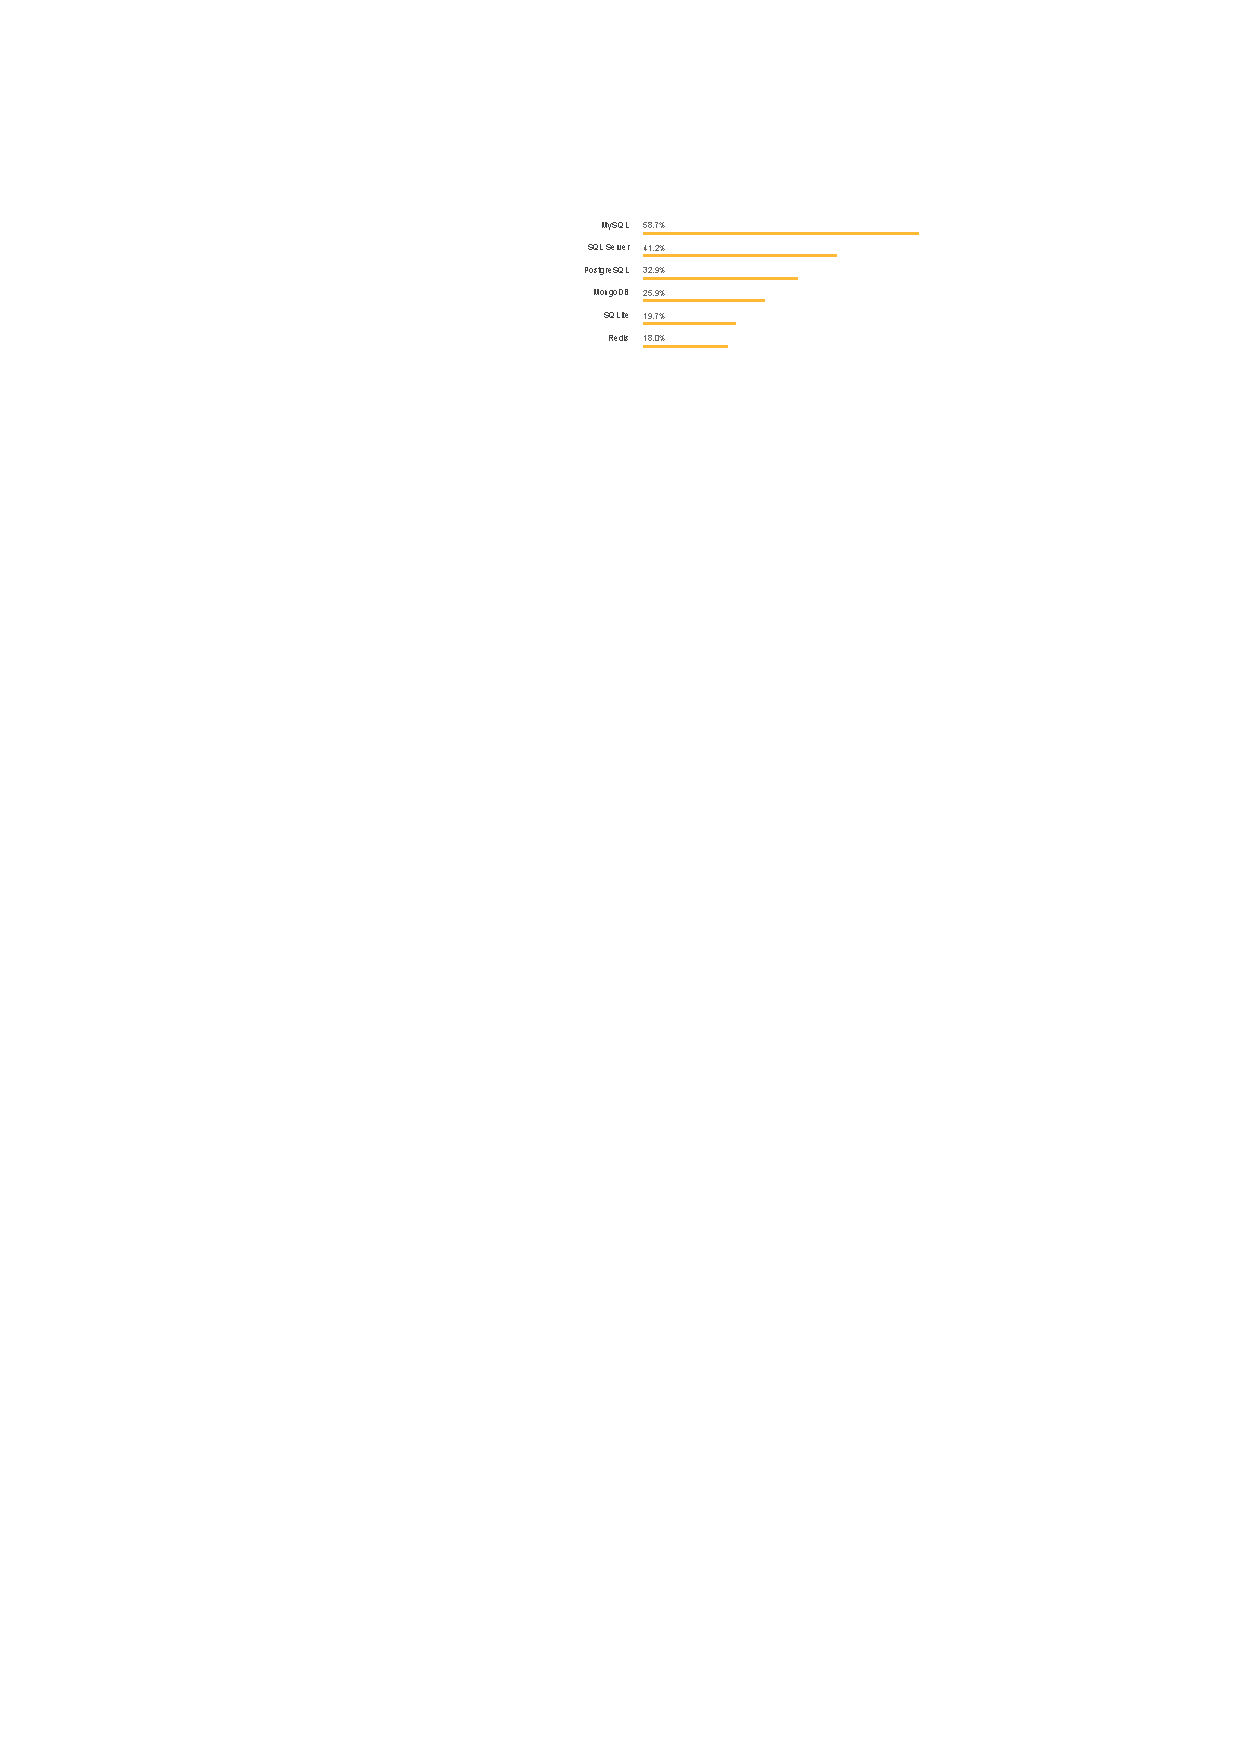
\includegraphics[width=0.9\textwidth]{img/stack-stats-db}
    	\caption[Popularita databází v roce 2018 dle průzkumu Stack Overflow]{Šest nejpopulárnějších databází v roce 2018 dle průzkumu Stack Overflow \cite{stack-stats18}}\label{fig:stack-stats18-db}
    \end{figure}
    
    MySQL \cite{db1}, SQLite \cite{db2} (která je velmi jednoduchá a často se např. používá pro prototypy aplikací) a SQL Server jsou relační databáze, PostgreSQL \cite{db3} je objektově relační databáze, všechny tedy sdílí tradiční práci s SQL (Structured Query Language). MongoDB \cite{db4} a Redis \cite{db5} jsou naproti tomu NoSQL databáze, jsou to moderní, flexibilní a škálovatelná řešení často se uplatňující v transakčně náročných aplikacích díky své rychlosti. MongoDB je dokumentová databáze a Redis databáze založená na formátu \enquote{klíč -- hodnota} a na využívání mezipaměti.
    
    
    \section{Srovnání hostingů}
    Je důležité rozlišit jednotlivé typy hostingů, kde může být aplikace uložena, pro tuto práci jsou možné 3 způsoby: tradiční hosting, PaaS a IaaS.
    
    Tradiční hosting je velmi populární hlavně díky své cenové dostupnosti a rozšířenosti, na serveru, který má nějakou konfiguraci, systém a komponenty, je každému uživateli vyhrazen jeho prostor \cite{hosting2}, často je nabízena funkcionalita emailů ad.
    
    PaaS (Platform as a service) a IaaS (Infrastructure as a Service) jsou podle \cite{hosting1} cloudové služby, které se od sebe liší mírou toho, co umožní uživateli, a co dělají za něj, společné mají to, že poskytnou uživateli virtuální prostředí. IaaS je prakticky pronájem hardwaru na dálku, nabízí zákazníkům plnou kontrolu nad vším od systému až po databází a aplikace. PaaS je v tomto ohledu striktnější a od poskytovatele dostanou uživatelé předpřipravené prostředí s mnoha doplněnými funkcemi včetně propojení s verzovacími systémy, mohou si vybrat konkrétní databázi a jazyk, ale nemají přístup k samotnému systému a dalším funkcím, díky tomu se ale mohou zaměřit na samotný vývoj aplikace, testování a nasazování.
    
        \subsection{Heroku}\label{heroku}
        Heroku od firmy Salesforce.com je PaaS služba, která podle \cite{heroku1} podporuje jazyky Ruby, PHP, Go, Python, Java, Scala, Clojure, technologii Node.js a jako výchozí databáze nabízí PostgreSQL a také Redis. Poskytuje několik programů, včetně jednoho zdarma \cite{heroku2}, ten má samozřejmě několik omezení:
            \begin{itemize}
                \item po 30~minutách neaktivity aplikace usíná a chvíli trvá, než se probudí,
                \item je k dispozici až 1~000~hodin provozu měsíčně pro jeden účet (to není problém, protože v rámci účtu neběží žádné další aplikace a 1~000~hodin je v přepočtu přes 41~dnů provozu na měsíc),
                \item maximálně 10~000~řádků v databázi PostgreSQL (rozšíření na 10~milionů stojí 9~\$ měsíčně).
            \end{itemize}
        Výhodou Heroku je, že i v programu zdarma dává možnost vybrat servery v Evropě \cite{heroku3}, také nabízí velkou škálu předpřipravených doplňků, díky kterým je možné aplikaci rozšířit o další funkcionalitu. Pokud by byl potřeba pokročilejší program mj. bez usínání aplikace, příplatek činí dalších 7~\$ měsíčně.
        
        \subsection{DigitalOcean}
        DigitalOcean je podle \cite{digitalocean1} služba IaaS poskytující distribuce Ubuntu, CentOS, Debian, Fedora, CoreOS a FreeBSD. Obsahuje spoustu předpřipravených možností a návodů, které usnadní start aplikace v typických prostředích. Servery má i v Evropě \cite{digitalocean2}. Nejlevnější řešení stojí podle \cite{digitalocean3} 5~\$ měsíčně.
        
        \subsection{Openshift}
        Openshift od firmy Red Hat je služba PaaS, která podle \cite{openshift1} umožňuje hostovat projekty v jazycích Java, Python, Perl, Ruby, PHP, technologiích .NET Core, Node.js na serverech Apache a Tomcat. Co se týče databází, nabízí MySQL, PostgreSQL, Redis, MariaDB a MongoDB. Má dva programy \cite{openshift2}: bezplatný a placený za 50~\$ měsíčně. Bezplatné hostování je především limitováno uspáním po 30~minutách neaktivity (probuzení chvíli trvá a zároveň spaní musí zabrat alespoň 18~hodin z každého 72hodinového intervalu), další nevýhodou bezplatné verze jsou servery umístěné v Severní Americe.
        
        \subsection{PythonAnyWhere}
        PythonAnyWhere je podle \cite{pythonanywhere1} a \cite{pythonanywhere2} Paas nabízející hosting pro aplikace v Pythonu -- zdarma umožňuje provozovat aplikace s omezeným výkonem a MySQL databází, vyšší výkon včetně dalších možností (např. PostgreSQL) lze získat za příplatek 5~\$ nebo více. Servery má v USA \cite{pythonanywhere3}.
        
        \subsection{Další možnosti}
        Dalšími možnostmi jsou například PaaS služba Google App Engine \cite{googleapp} a IaaS služba od Amazon Web Services s názvem EC2 \cite{aws1}, obě mají velmi rozsáhlé ceníky se spoustou pokročilých variant včetně kalkulátorů a není lehké se v nich vyznat (například AWS dává k dispozici 12 měsíců s určitými podmínkami zdarma, ale při jejich překročení nebo vypršení roční lhůty přesune uživatele do placeného programu bez možnosti návratu \cite{aws2}). Také je potřeba zmínit český hosting Roští, který podle \cite{rosti} nabízí hosting aplikací v Pythonu, Ruby, PHP a Node.js, nabízí relativně levný program za 99~Kč měsíčně. Vzhledem k tomu, že už jsem našel rozumné varianty (dokonce i zdarma), které pro rozjezd projektu postačí, nebudu se těmito službami hlouběji v této práci zaobírat.

    \section{Zvolené řešení}\label{reseni}
    Na úvod bych chtěl krátce uvést své zkušenosti s technologiemi v oblasti webových aplikací. V minulosti jsem si vyzkoušel práci s Javou a Servlety, častěji jsem také pracoval s čistým PHP, nikdy jsem ale nepracoval s frameworky. Na základě těchto zkušeností jsem se rozhodl zvolit pro tuto práci nějaký framework, který mi usnadní práci. Co se týče klientské části, zde jsem pracoval s čistým JS a případně jQuery, vzhledem k pokročilejší interaktivitě aplikace v rámci této práce a na základě předchozích zkušeností jsem chtěl využít služby frameworku/knihovny i na straně klienta. V oblasti databází jsem pracoval především s MySQL a PostgreSQL. Co se týče hostingů, mám zkušenosti s klasickými tuzemskými hostingy, tedy kombinace Apache, PHP, MySQL, z týmového projektu také mám zkušenosti s Heroku.
    
    Při volbě technologií jsem také využil možnost vidět díky projektu RealWorld\footnote{\url{https://github.com/gothinkster/realworld}} reálnou aplikaci včetně kódu využívající různé serverové a klientské technologie. Jak autor popisuje v \cite{realworld}, rozhodli se tento projekt vytvořit především kvůli rychle se rozvíjejícímu odvětví webových technologií a prakticky nemožnosti zmapovat najednou všechny technologie jedním člověkem -- existovaly sice projekty ukazující tímto způsobem v mnoha technologiích vytvořenou aplikaci na správu úkolů, ale takovýto typ aplikace se většinou liší od CRUD aplikace, kterou většina lidí vytvoří, zvolili tedy blog. Díky tomu se na jejich repozitáři nachází implementované aplikace v různých jazycích a frameworcích, a to jak pro klientskou část, tak pro serverovou, a na dalších technologiích se už pracuje \cite{realworld-git}.
    
    Na základě všech informací zjištěných během této rešerše a dalšího hledání jsem se rozhodl využít na serverovou část Python 3 s frameworkem Django (v čerstvě vydané verzi 2.0 z prosince 2017, která mj. výrazně zjednodušuje zápis URL routování \cite{django2}) a React na klientské části (JS a JSX spolu s HTML a CSS) komunikující skrze API vystavené serverem. Klientská část bude realizovaná konceptem SPA a pro začátek bude využívat renderování pouze na straně klienta. Python s Djangem je velmi populární volbou pro spoustu projektů (viz. např. \cite{stack-stats18}).
    
    Python jsem zvolil, protože se jedná o stále více populární jazyk a díky této práci tak budu mít možnost se ho naučit (podle průzkumu Jetbrains \cite{jetbrains-stats} je to jazyk, který by se chtělo naučit nebo na něj přímo přejít nejvíce programátorů, ke stejnému názoru došel i průzkum Stack Overflow \cite{stack-stats18}, kde je vidět, že patří Python patří do trojice nejvíce oblíbených jazyků dle osobních preferencí) a vyzkoušet si jeho jednoduchou syntaxi a práci s ním. Django jsem zvolil z několika důvodů, zaprvé mě při procházení dokumentací jeho dokumentace zaujala svou rozsáhlostí a poměrně přátelským přístupem, zadruhé se jedná o \enquote{batteries included} framework a protože na klientské části bude React, který je přesným opakem (tedy obsahuje jen nutný základ a je na uživateli, co zvolí dalšího), rozhodl jsem se zvolit jeden přístup na straně klienta a druhý přístup na straně serveru.
    
    React jsem zvolil především kvůli jeho relativně stabilní architektuře \cite{js-fw2}, Angular se výrazně proměnil a vznikl Angular 2 s architekturou bližší Reactu (viz. podsekce \ref{sec:angular}), ale dostupné návody, články a literatura je spíše pro starší AngularJS (často jsou tyto názvy zaměňovány, což je docela matoucí pro nově příchozího). Volba také souvisela s Djangem, kdy jsem chtěl zkusit využít pro klientskou část spíše modulárnější technologii i vzhledem k častěji se měnícího UI oproti serverové části. VueJS jsem nezvolil kvůli jeho menší rozšířenosti a nejistotě budoucnosti (není za ním firma).
    
    Protože cílem této práce má být jednoduchá a uživateli srozumitelná aplikace, je třeba poskytnout mu co nejlepší uživatelský prožitek a zkušenost, z toho důvodu je zvolen přístup SPA, který je často ve spojení s JS frameworky používán (viz. podsekce \ref{spampa}).
    
    Jako databázi použiji PostgreSQL, protože se jedná o základní databázi, kterou poskytuje Heroku, které bylo na základě srovnání vybráno jako nejvhodnější hosting (může být zdarma i se servery v Evropě a zároveň s ním mám už zkušenosti z jiného projektu).